\documentclass{article}
\usepackage[utf8]{inputenc}
\usepackage{algorithm}
\usepackage{algpseudocode}
\usepackage{amsmath, amsfonts, amssymb}
\usepackage[braket, qm]{qcircuit}
\usepackage{tikz}
\usetikzlibrary{calc}

\algrenewcommand\algorithmicrequire{\textbf{Input:}}
\algrenewcommand\algorithmicensure{\textbf{Output:}}

\makeatletter
\renewcommand{\fnum@algorithm}{\fname@algorithm}
\makeatother

\begin{document}
\pagestyle{empty}

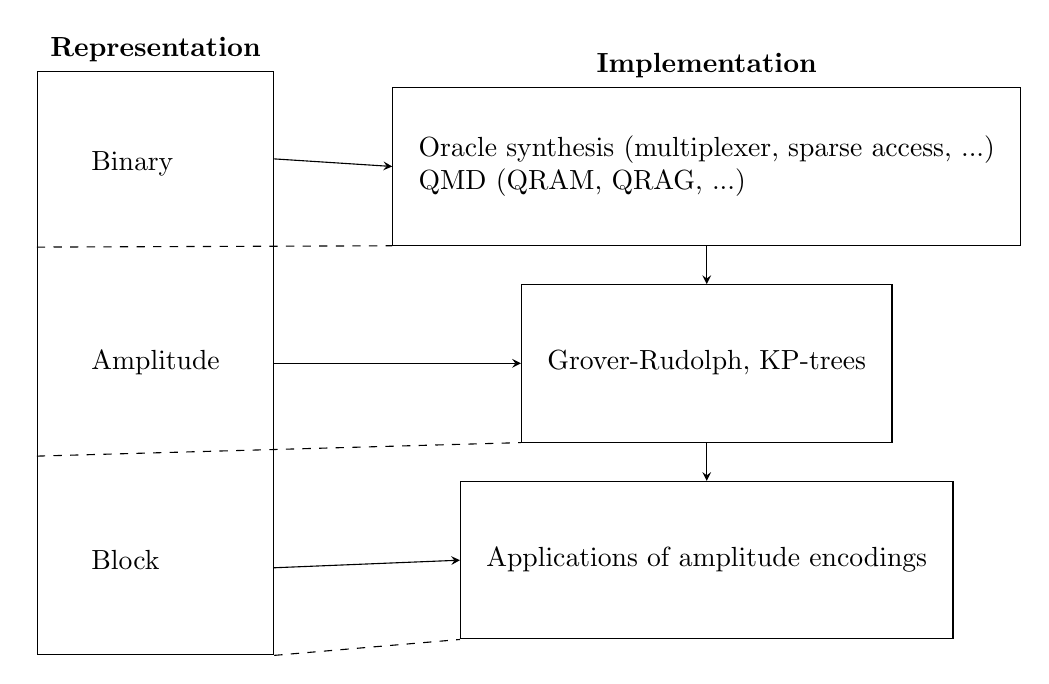
\begin{tikzpicture}

% Encoding
\node[draw, minimum width=3cm, minimum height=2cm] (encbox) at (0,-5) {
\begin{tabular}{l}
        \; \\
        \; \\
        Binary\\
        \; \\
        \; \\
        \; \\
        \; \\
         \; \\
        Amplitude\\
        \; \\
        \; \\
        \; \\
        \; \\
        \; \\
        Block \\
        \; \\
        \; \\
    \end{tabular}
};
\node[above] at (encbox.north) {\textbf{Representation}};

% Binary
\node[draw, minimum width=3cm, minimum height=2cm] (numbox) at (7,-2.5) {
\begin{tabular}{l}
        Oracle synthesis (multiplexer, sparse access, ...) \\
         QMD (QRAM, QRAG, ...) 
    \end{tabular}
};
\node[above] at (numbox.north) {\textbf{Implementation}};

% Vector
\node[draw, minimum width=3cm, minimum height=2cm] (vecbox) at (7,-5) {
\begin{tabular}{l}
        Grover-Rudolph, KP-trees
    \end{tabular}
};

% Matrices
\node[draw, minimum width=3cm, minimum height=2cm] (matbox) at (7,-7.5) {
\begin{tabular}{l}
        Applications of amplitude encodings\\
            \end{tabular}
};

% Calculate midpoint of the second arrow
\coordinate (midup) at ($(encbox.east)!0.7!(encbox.north east)$);
\coordinate (middown) at ($(encbox.east)!0.7!(encbox.south east)$);

% Arrows
\draw[->, >=stealth] (vecbox.south) -- (matbox.north) node[midway, above] {};
\draw[->, >=stealth] (numbox.south) -- (vecbox.north) node[midway, above] {};

\draw[->, >=stealth] (midup) -- (numbox.west) node[midway, above] {};
\draw[->, >=stealth] (encbox.east) -- (vecbox.west) node[midway, above] {};
\draw[->, >=stealth] (middown) -- (matbox.west) node[midway, above] {};

% Horizontal Line Numbers
\def\lineheightNumbers{42}
%\draw[dashed] ([xshift=-1.5cm,yshift=\lineheightNumbers]encbox.west) node[right, above] {\;\;\;\;\;\;\;\;\;\;\;\;\;Numbers}-- ([xshift=0cm,yshift=0]numbox.south west);
\draw[dashed] ([yshift=\lineheightNumbers]encbox.west) node[right, above] {}-- ([xshift=0cm,yshift=0]numbox.south west);


% Horizontal Line Vectors
\def\lineheightVectors{72}
%\draw[dashed] ([xshift=-1.5cm,yshift=\lineheightVectors]encbox.south west)node[right, above] {\;\;\;\;\;\;\;\;\;\;\;\;\;Vectors} -- ([xshift=0cm]vecbox.south west);
\draw[dashed] ([yshift=\lineheightVectors]encbox.south west)node[right, above] {} -- ([xshift=0cm]vecbox.south west);

% Horizontal Line Matrices
\def\lineheightMatrices{0}
%\draw[dashed] ([xshift=-1.5cm,yshift=\lineheightMatrices]encbox.south west)node[right, above] {\;\;\;\;\;\;\;\;\;\;\;\;\;Matrices} -- ([xshift=0cm,yshift=\lineheightMatrices]matbox.south west);
\draw[dashed] ([yshift=\lineheightMatrices]encbox.south east)node[right, above] {} -- ([xshift=0cm,yshift=\lineheightMatrices]matbox.south west);
\end{tikzpicture}

\end{document}
